\documentclass[a4paper, top=10mm]{article}
%for writing from the top
\usepackage{fullpage}
%for math
\usepackage{amsmath}
\usepackage{mathrsfs}
\usepackage{amsthm}
%for images
\usepackage{graphicx}
%for color
\usepackage{xcolor}
%for title
\title{\textbf{\huge{A Christmas Elf...}}}
\author{Enigma n\textsuperscript{o}4}
\date{14\textsuperscript{th} December 2023}

\newtheorem*{hint}{Hint}

\addtolength{\voffset}{-2cm}
\addtolength{\textheight}{5cm}


\begin{document}
	\maketitle
	
	A Christmas elf in the upper left corner (square "A") moves across the grid squares.
	He needs to avoid the two squares occupied by wolves.
	He can only jump to one of the squares adjacent to the one he is on.
	He cannot jump diagonally.
	
	\begin{center}
		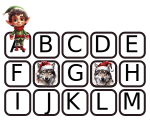
\includegraphics[width=\linewidth]{04map.png}\\
	\end{center}
	
	\textbf{The elf will perform $2023$ jumps.
	List all the squares he may reach.}
	
	NB: Enter the (capital) letter(s) in alphabetical order, with no space nor punctuation between them.
	
	% BDFGHJL
	
\end{document}